\documentclass[a4paper,11pt]{jsarticle}


% 数式
\usepackage{amsmath,amsfonts,amssymb}
\usepackage{bm}
% 画像
\usepackage[dvipdfmx]{graphicx}
\usepackage{siunitx}
\usepackage{wrapfig}
\usepackage{cases}
\makeatletter
\newcommand{\figcaption}[1]{\def\@captype{figure}\caption{#1}}
\newcommand{\tblcaption}[1]{\def\@captype{table}\caption{#1}}
\makeatother


\begin{document}

\title{自主ゼミ用資料}
\author{平林広}
\date{\today}
\maketitle

\section{保存力のみ}

\subsection{自由落下}

ラグランジュの運動方程式
\begin{align*}
  \frac{d}{dt}\frac{\partial L}{\partial \dot{x}} - \frac{\partial L}{\partial x} = 0
\end{align*}
\begin{align*}
  L = T - U \quad (T:運動エネルギー, U:位置エネルギー)
\end{align*}
を説明する。

まずは自由落下
\begin{align*}
  m\ddot{x} = -m\cdot g
\end{align*}
から計算してみる。
\begin{figure}[b]
  \centering
  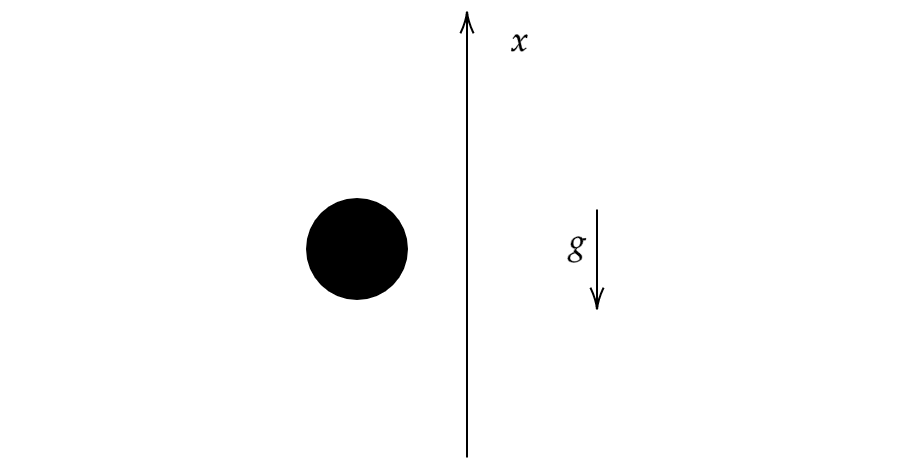
\includegraphics[width = 0.7\textwidth]{20210514_Freefall.png}
  \caption{設定}
  \label{}
\end{figure}
\begin{align*}
  T &= \frac{1}{2}m\dot{x}^2
  \\ U & = m\cdot g\cdot x
\end{align*}
であるから
\begin{align*}
  L = \frac{1}{2}m\dot{x}^2 - mgx
\end{align*}
頑張って計算を進めると
\begin{align*}
  \frac{d}{dt}\frac{\partial L}{\partial \dot{x}} 
  &= \frac{d}{dt}\frac{\partial }{\partial \dot{x}}\left(\frac{1}{2}m\dot{x}^2 - mgx\right)
  \\ &= \frac{d}{dt}\left(m\dot{x}\right)
  \\ &= m\ddot{x}
\end{align*}
\begin{align*}
  \frac{\partial L}{\partial x}
  &= \frac{\partial }{\partial x}\left(\frac{1}{2}m\dot{x}^2 - mgx\right)
  \\ &= - mg
\end{align*}
\begin{align*}
  \therefore \frac{d}{dt}\frac{\partial L}{\partial \dot{x}} - \frac{\partial L}{\partial x}
  &= m\ddot{x} - \left(-mg\right)
  \\ &= m\ddot{x} + mg
\end{align*}
よってラグランジュ方程式は
\begin{align*}
  \frac{d}{dt}\frac{\partial L}{\partial \dot{x}} - \frac{\partial L}{\partial x} = 0
\end{align*}
\begin{align*}
  \Leftrightarrow m\ddot{x} + mg = 0
\end{align*}
\begin{align*}
  \Leftrightarrow m\ddot{x} = -m\cdot g
\end{align*}

\subsection{単振り子}

次は座標変換も含むやつ
\begin{figure}[t]
  \centering
  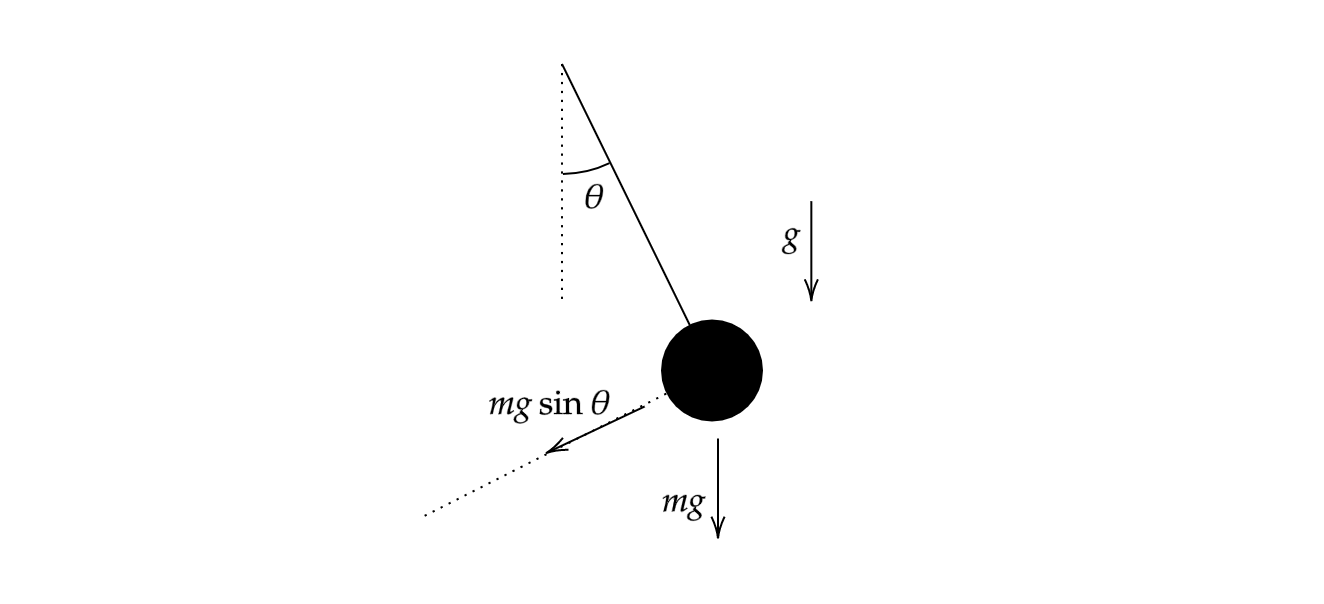
\includegraphics[width = 1\textwidth]{20210514_Single_Pendulumpng.png}
  \caption{単振り子}
  \label{}
\end{figure}
今回も相変わらず
\begin{align*}
  T &= \frac{1}{2}m\left(\dot{x}^2 + \dot{y}^2\right)
  \\ U & = m\cdot g\cdot y
\end{align*}
だが、拘束条件
\begin{align*}
  x^2 + y^2 = r
\end{align*}
とか
\begin{align*}
  \begin{cases}
    x = r\sin\theta \\
    y = -r\cos\theta
  \end{cases}
\end{align*}
とかがある。
どれを選ぶかは自由。
$\theta$と結び付けたいから後者。
\begin{align*}
  T &= \frac{1}{2}m\left[(r\dot{\theta}\cos\theta)^2 + (r\dot{\theta}\sin\theta)^2\right]
  \\ &= \frac{1}{2}mr^2\dot{\theta}^2
  \\ U & = m\cdot g\cdot y
  \\ &= -mgr\cos\theta
  \\ \therefore L &= T - U
  \\ &= \frac{1}{2}mr^2\dot{\theta}^2 + mgr\cos\theta
\end{align*}
頑張って計算を進めると
\begin{align*}
  \frac{d}{dt}\frac{\partial L}{\partial \dot{\theta}} 
  &= \frac{d}{dt}\frac{\partial }{\partial \dot{\theta}}\left(\frac{1}{2}mr^2\dot{\theta}^2 + mgr\cos\theta\right)
  \\ &= mr^2\ddot{\theta}
\end{align*}
\begin{align*}
  \frac{\partial L}{\partial \theta}
  &= \frac{\partial }{\partial \theta}\left(\frac{1}{2}mr^2\dot{\theta}^2 + mgr\cos\theta\right)
  \\ &= - mgr\sin\theta
\end{align*}
\begin{align*}
  \therefore \frac{d}{dt}\frac{\partial L}{\partial \dot{\theta}} - \frac{\partial L}{\partial \theta}
  &= mr^2\ddot{\theta} - \left(-mgr\sin\theta\right)
  \\ &= mr^2\ddot{\theta} + mgr\sin\theta
\end{align*}
よってラグランジュ方程式は
\begin{align*}
  \frac{d}{dt}\frac{\partial L}{\partial \dot{\theta}} - \frac{\partial L}{\partial \theta} = 0
\end{align*}
\begin{align*}
  \Leftrightarrow mr^2\ddot{\theta} + mgr\sin\theta = 0
\end{align*}
\begin{align*}
  \Leftrightarrow mr^2\ddot{\theta} = -mgr\sin\theta
\end{align*}
\begin{align*}
  \Leftrightarrow mr\ddot{\theta} = -mg\sin\theta
\end{align*}

\section{保存力以外あり}

\subsection{方程式自体の変化}

保存力がないと考えると、
\begin{align*}
  \frac{d}{dt}\frac{\partial L}{\partial \dot{x}} - \underbrace{\frac{\partial L}{\partial x}}_{=0} = ?
\end{align*}
\begin{align*}
  \therefore\frac{d}{dt}\frac{\partial L}{\partial \dot{x}} = ?
\end{align*}
\begin{align*}
  \therefore m\ddot{x} = ?
\end{align*}
自由落下とかだとこれが単純で$-mg$になる。

\subsection{?の正体}

xy座標での力の表し方はとても簡単で素晴らしいが、
単振り子のようにほかの変数のほうが表しやすいような場合もある。
その時に、その表したい変数に対応する力的なものが計算できるとありがたい。
この力的なもののことを一般化力という。

\[
  エネルギーが一致するように、一般化力を定める
\]
この考えに基づいて、
安藤さんと似たようなことを考える。

直交座標系$x_1, x_2, \cdots$で
微小に変位が起きた時のエネルギー変化は
\[
  \delta W = \sum_i F_i\delta x_i
\]
と表される。
変な座標系$\theta_1, \theta_2, \cdots$を用いると偏微分的に
\[
  \delta x_i = \sum_j \frac{\partial x_i}{\partial \theta_j}\delta \theta_j
\]
となる(これが分からない場合はホワイトボードで解説予定)。
だから
\begin{align*}
  \delta W &= \sum_i F_i\delta x_i
  \\ &= \sum_i F_i\left(\sum_j \frac{\partial x_i}{\partial \theta_j}\delta \theta_j\right)
  \\ &= \sum_i \sum_j F_i\frac{\partial x_i}{\partial \theta_j}\delta \theta_j
  \\ &= \sum_j 
  \underbrace{\left(\sum_i F_i\frac{\partial x_i}{\partial \theta_j}\right)}_{=\Theta_jとする}
  \delta \theta_j
  \\ &= \sum_j \Theta_j\delta \theta_j
\end{align*}
ってなって、いい感じかもしれない$\Theta_j$が得られる。

例えば単振り子だと
\begin{align*}
  F_x &= 0
  \\ F_y &= -mg
\end{align*}
だったから
\begin{align*}
  \Theta &= F_x \frac{\partial x}{\partial \theta} + F_y \frac{\partial y}{\partial \theta}
  \\ &= F_x r\sin\theta + F_y r\sin\theta
  \\ &= -mgr\sin\theta
\end{align*}
となる。
実はこれ、重力の固定点周りのトルクと一致している。
角速度とトルクの積がパワーとなることを考えれば、理解できるはず。

こんな感じで単振り子の重力をポテンシャルとして考えなくても、
\begin{align*}
  \frac{d}{dt}\frac{\partial L}{\partial \dot{\theta}} 
  - \underbrace{\frac{\partial L}{\partial \theta}}_{0} = \Theta
\end{align*}
\begin{align*}
  \therefore mr^2\ddot{\theta} = -mgr\sin\theta
\end{align*}
\begin{align*}
  \Leftrightarrow mr\ddot{\theta} = -mg\sin\theta
\end{align*}
となって、簡単に運動方程式が求まる。

\subsection{トルクを力に変換}
\begin{figure}[t]
  \centering
  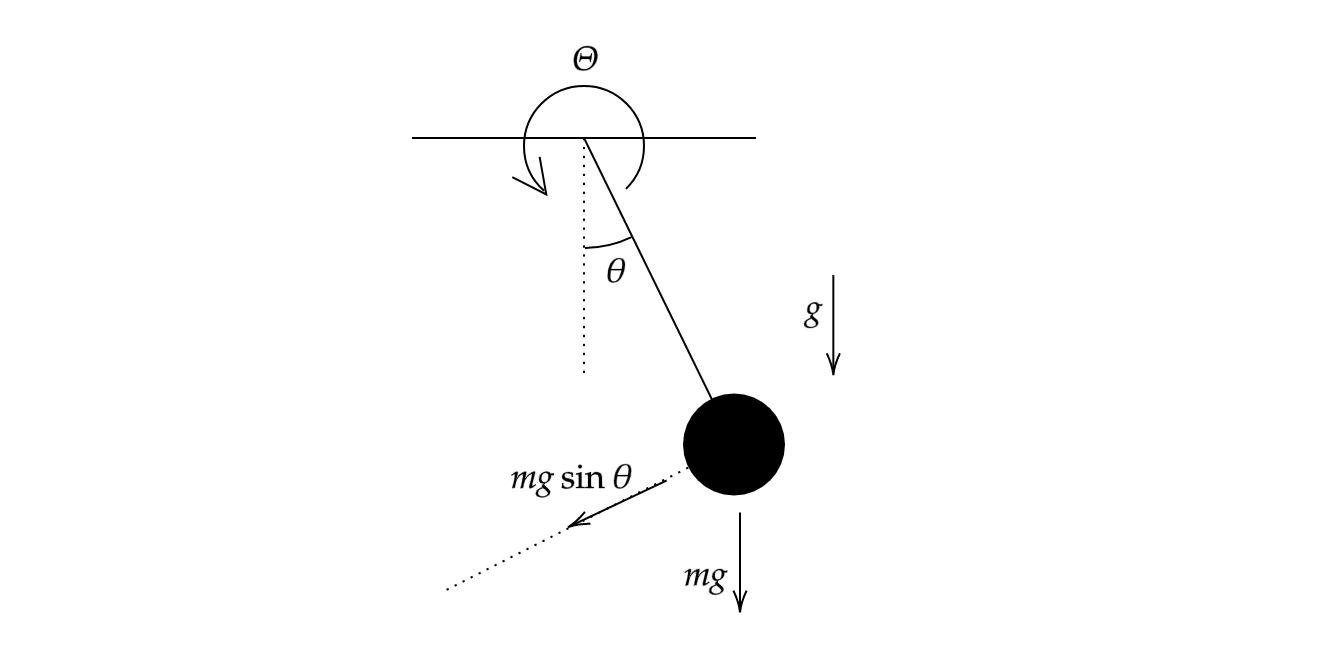
\includegraphics[width = 0.8\textwidth]{20210514_Single_Pendulumpng_With_Tau.png}
  \caption{}
  \label{}
\end{figure}
$(x,y)$を極座標表示するとき、変数は$(r,\theta)$だから、
\begin{align*}
  \begin{cases}
    \displaystyle F_x = \Theta \frac{\partial \theta}{\partial x} + \mathbb{R} \frac{\partial r}{\partial x}
    \\
    \\ \displaystyle F_y = \Theta \frac{\partial \theta}{\partial y} + \mathbb{R} \frac{\partial r}{\partial x}
  \end{cases}
\end{align*}
だから
\begin{align*}
  \frac{\partial \theta}{\partial x}, \frac{\partial \theta}{\partial y}
\end{align*}
を計算しなくちゃいけない。これが少し面倒。

\begin{align*}
  \begin{cases}
    x = r\sin\theta \\
    y = -r\cos\theta
  \end{cases}
\end{align*}
の時に
\begin{align*}
  \frac{\partial }{\partial r} &= 
  \frac{\partial x}{\partial r} \frac{\partial }{\partial x}
  + \frac{\partial y}{\partial r}\frac{\partial }{\partial y}
  \\ 
  \frac{\partial }{\partial \theta} &= 
  \frac{\partial x}{\partial \theta} \frac{\partial }{\partial x}
  + \frac{\partial y}{\partial \theta}\frac{\partial }{\partial y}
\end{align*}
ちょっと計算して
\begin{align*}
  \frac{\partial }{\partial r} &= 
  \sin\theta \frac{\partial }{\partial x}
  -\cos\theta\frac{\partial }{\partial y} \tag*{(1)}
  \\ 
  \frac{\partial }{\partial \theta} &= 
  r\cos\theta \frac{\partial }{\partial x}
  + r\sin\theta\frac{\partial }{\partial y} \tag*{(2)}
\end{align*}
連立方程式を頑張って計算する。一個目
\begin{align*}
  r\sin\theta \frac{\partial }{\partial r} &= r\sin^2\theta \frac{\partial }{\partial x} - r\sin\theta\cos\theta \frac{\partial }{\partial y} \tag*{(1)$\times r\sin\theta$}
  \\ \cos\theta \frac{\partial }{\partial \theta} &= r\cos^2\theta \frac{\partial }{\partial x} + r\sin\theta\cos\theta \frac{\partial }{\partial y} \tag*{(2)$\times \cos\theta$}
\end{align*}
\begin{align*}
  &\therefore r \frac{\partial }{\partial x} = r\sin\theta \frac{\partial }{\partial r} + \cos\theta \frac{\partial }{\partial \theta}
  \\& \therefore \frac{\partial }{\partial x} = \sin\theta \frac{\partial }{\partial r} + \frac{\cos\theta}{r} \frac{\partial }{\partial \theta}
\end{align*}
二個目
\begin{align*}
  r\cos\theta \frac{\partial }{\partial r} &= r\sin\theta\cos\theta \frac{\partial }{\partial x} - r\cos^2\theta \frac{\partial }{\partial y} \tag*{(1)$\times r\cos\theta$}
  \\ \sin\theta \frac{\partial }{\partial \theta} &= r\sin\theta\cos\theta \frac{\partial }{\partial x} + r\sin^2\theta\ \frac{\partial }{\partial y} \tag*{(2)$\times \sin\theta$}
\end{align*}
\begin{align*}
  &\therefore r \frac{\partial }{\partial y} = -r\cos\theta \frac{\partial }{\partial r} + \sin\theta \frac{\partial }{\partial \theta}
  \\& \therefore \frac{\partial }{\partial y} = -\cos\theta \frac{\partial }{\partial r} + \frac{\sin\theta}{r} \frac{\partial }{\partial \theta}
\end{align*}
よって
\begin{align*}
  \frac{\partial }{\partial x} &= \sin\theta \frac{\partial }{\partial r} + \frac{\cos\theta}{r} \frac{\partial }{\partial \theta}
  \\ \frac{\partial }{\partial y} &= -\cos\theta \frac{\partial }{\partial r} + \frac{\sin\theta}{r} \frac{\partial }{\partial \theta}
\end{align*}
よって
\begin{align*}
  F_x = \Theta \frac{\partial \theta}{\partial x} + \mathbb{R}\frac{\partial r}{\partial x}
  = \Theta \frac{\cos\theta}{r} + \mathbb{R}\sin\theta
\end{align*}
\begin{align*}
  F_y = \Theta \frac{\partial \theta}{\partial r} + \mathbb{R}\frac{\partial r}{\partial y}
   = \Theta \frac{\sin\theta}{r} - \mathbb{R} \cos\theta
\end{align*}
だが、
$\Theta$由来の$F_x, F_y$である$F_x^\Theta, F_y^\Theta$
\begin{align*}
  F_x^\Theta = \Theta \frac{\partial \theta}{\partial x}
   = \Theta \frac{\cos\theta}{r}
\end{align*}
\begin{align*}
  F_y^\Theta = \Theta \frac{\partial \theta}{\partial r}
   = \Theta \frac{\sin\theta}{r}
\end{align*}
これがちょうどこんな方向になる。
\begin{figure}[h]
  \centering
  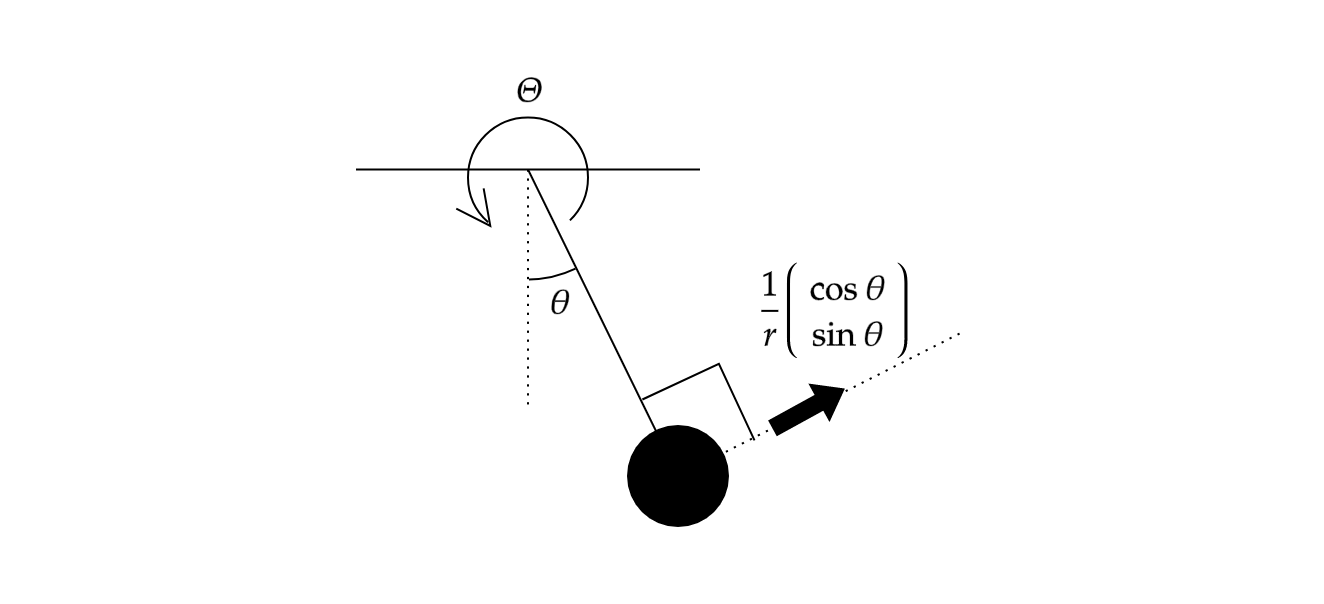
\includegraphics[width = 1\textwidth]{20210514_Single_Pendulumpng_With_Tau_Force.png}
  \caption{}
  \label{}
\end{figure}
固定点周りのトルクを計算しなおしても
\begin{align*}
  r\cos\theta \times F_x^\Theta + r\sin\theta \times F_y^\Theta = r\cos\theta \times \Theta \frac{\cos\theta}{r} + r\sin\theta\times\Theta\frac{\sin\theta}{r}
  = \Theta
\end{align*}
てなって整合性は取れている。

\section{トルクと外力}
\begin{figure}[b]
  \centering
  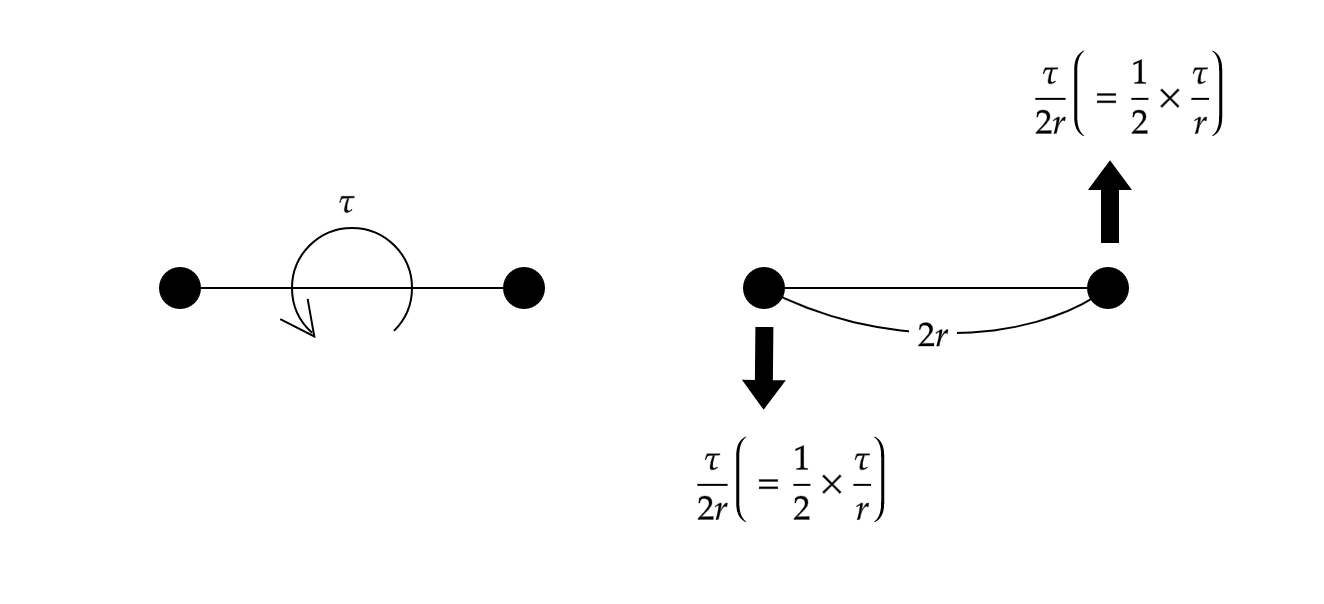
\includegraphics[width = 1\textwidth]{Torque_Force.png}
  \caption{}
  \label{fig:Torque_Force}
\end{figure}
あるセグメントにトルクをかけることは基本的に図\ref{fig:Torque_Force}みたいな感じ。
トルクは日本語だと偶力っていうくらいだから、
大きさ同じで、方向が正反対で、作用位置が違う力。
大きさ同じで方向が逆だから重心は動かさない。

\begin{figure}[t]
  \centering
  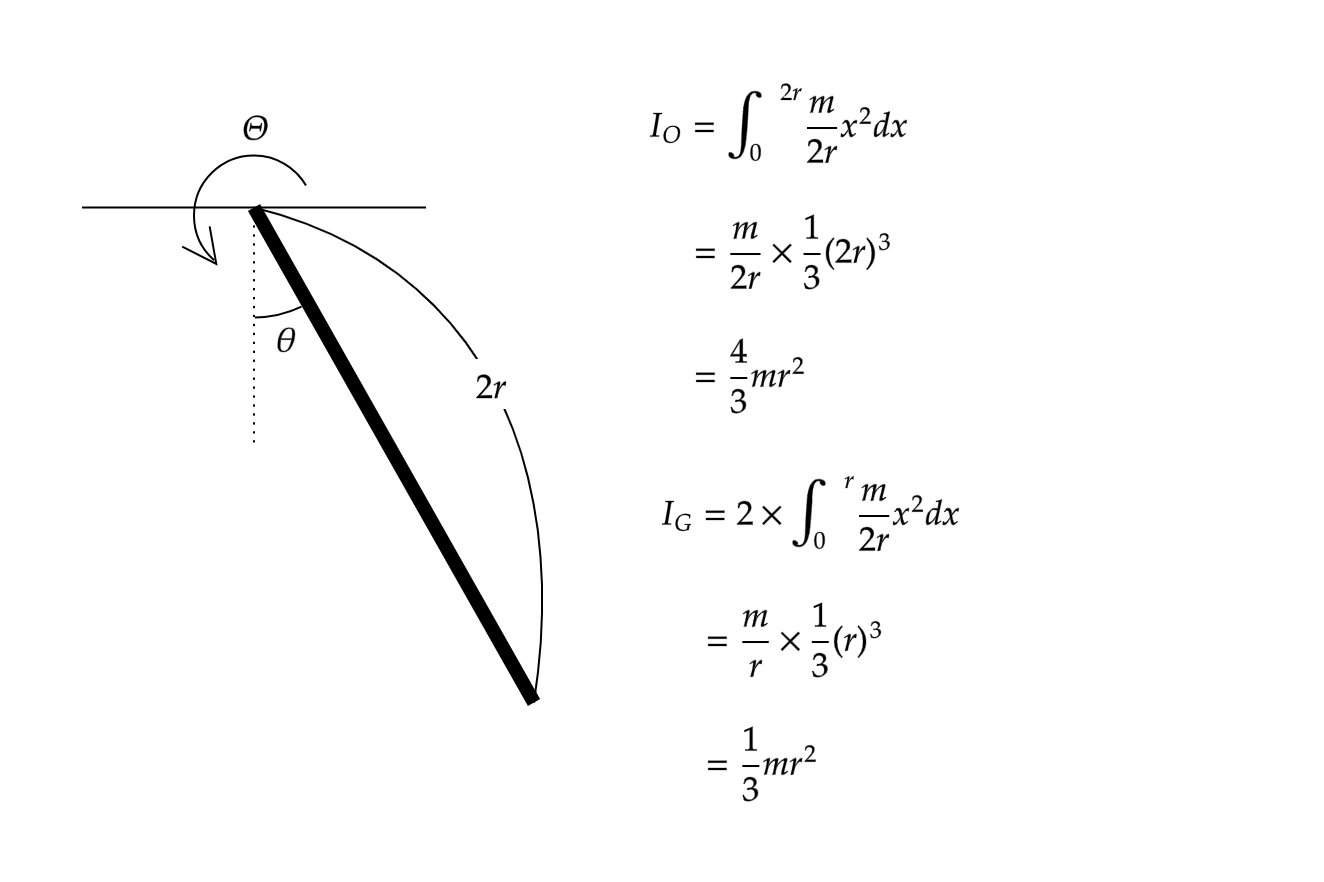
\includegraphics[width = 1\textwidth]{Single_Stick.png}
  \caption{}
  \label{fig:Single_Stick}
\end{figure}
でも図\ref{fig:Single_Stick}だと、
トルクによって棒が持ち上がるから、
重心が動いている。
しかも重心周りの角力積も$\Theta\times (作用時間)$に一致しない。
これは実はトルクによって固定点に力が発生しているからである。
実感を得るためにも、固定点に発生する力を計算してみよう。

\subsection{拘束力の計算}
拘束力の計算はラグランジアン的には以下の手順に従う。
\begin{enumerate}
  \item 拘束がない状態での運動方程式を立てる
  \item 拘束する変数が0になるような一般化力を求める
\end{enumerate}

\begin{figure}[t]
  \centering
  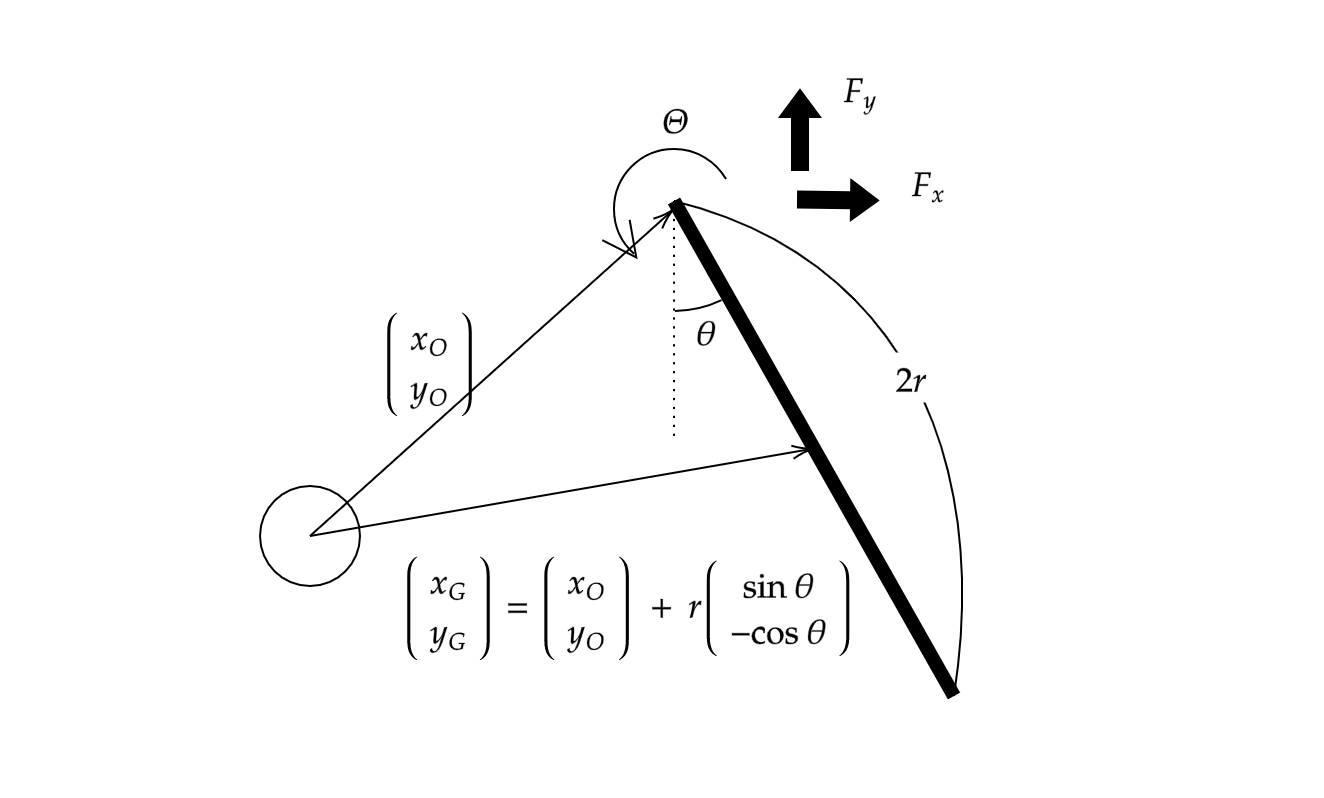
\includegraphics[width = 1\textwidth]{007.png}
  \caption{}
  \label{fig:007}
\end{figure}
拘束がない状態とは図\ref{fig:007}みたいな感じ。
$x,y$に関しても微分したりする。結構大変。

頑張りフェーズスタート

\begin{align*}
  T = \frac{1}{2}m(\dot{x}_G{}^2 + \dot{y}_G{}^2) + \frac{1}{2}I_G \dot{\theta}^2
\end{align*}
\begin{align*}
  U = 0
\end{align*}
だから$\dot{x}_G,\dot{y}_G$を計算する必要がある。

\begin{align*}
  \dot{x}_G &= \dot{x}_O + r\dot{\theta}\cos\theta
  \\ \dot{y}_G &= \dot{y}_O + r\dot{\theta}\sin\theta
\end{align*}
\begin{align*}
  \therefore 
  \dot{x}_G{}^2 &= \dot{x}_O{}^2 + r^2\dot{\theta}^2\cos^2\theta + 2r\dot{x}_O\dot{\theta}\cos\theta
  \\ \dot{y}_G{}^2 &= \dot{y}_O{}^2 + r^2\dot{\theta}^2\sin^2\theta + 2r\dot{y}_O\dot{\theta}\sin\theta
\end{align*}
\begin{align*}
  \therefore \dot{x}_G{}^2 + \dot{y}_G{}^2 = \dot{x}_O{}^2 + \dot{y}_O{}^2 + r^2\dot{\theta}^2 + 2r\dot{x}_O\dot{\theta}\cos\theta + 2r\dot{y}_O\dot{\theta}\sin\theta
\end{align*}
\begin{align*}
  \therefore L = T &= \frac{1}{2}m(\dot{x}_G{}^2 + \dot{y}_G{}^2) + \frac{1}{2}I_G \dot{\theta}^2
  \\ & = \frac{1}{2}m\left(\dot{x}_O{}{}^2 + \dot{y}_O{}^2 + r^2\dot{\theta}^2 + 2r\dot{x}_O\dot{\theta}\cos\theta + 2r\dot{y}_O\dot{\theta}\sin\theta\right) + \frac{1}{2}I_G \dot{\theta}^2
\end{align*}

\begin{align*}
  \frac{\partial L}{\partial x_O} = 0
\end{align*}
\begin{align*}
  \frac{\partial L}{\partial \dot{x}_O} = m\dot{x}_O + mr\dot{\theta}\cos\theta
\end{align*}
\begin{align*}
  \frac{d}{dt}\frac{\partial L}{\partial \dot{x}_O} = m\ddot{x}_O + mr\ddot{\theta}\cos\theta - mr\dot{\theta}^2\sin\theta
\end{align*}

\begin{align*}
  \frac{\partial L}{\partial y_O} = 0
\end{align*}
\begin{align*}
  \frac{\partial L}{\partial \dot{y}_O} = m\dot{y}_O + mr\dot{\theta}\sin\theta
\end{align*}
\begin{align*}
  \frac{d}{dt}\frac{\partial L}{\partial \dot{y}_O} = m\ddot{y}_O + mr\ddot{\theta}\sin\theta + mr\dot{\theta}^2\cos\theta
\end{align*}

\begin{align*}
  \frac{\partial L}{\partial \theta} = -mr\dot{x}_O\dot{\theta}\sin\theta + mr\dot{y}_O\dot{\theta}\cos\theta
\end{align*}
\begin{align*}
  \frac{\partial L}{\partial \dot{\theta}} = mr^2\dot{\theta} + r\dot{x}_O\cos\theta + r\dot{y}_O\sin\theta + I_G\dot{\theta}
\end{align*}
\begin{align*}
  \frac{d}{dt}\frac{\partial L}{\partial \dot{\theta}} = mr^2\ddot{\theta} + r\ddot{x}_O\cos\theta 
  + r\dot{x}_O\dot{\theta}\cos\theta + r\ddot{y}_O\sin\theta - r\dot{y}_O\dot{\theta}\cos\theta + I_G\ddot{\theta}
\end{align*}

\begin{align*}
  \begin{cases}
    F_x = m\ddot{x}_O + mr\ddot{\theta}\cos\theta - mr\dot{\theta}^2\sin\theta
    \\ F_y = m\ddot{y}_O + mr\ddot{\theta}\sin\theta + mr\dot{\theta}^2\cos\theta
    \\ \Theta = mr^2\ddot{\theta} + r\ddot{x}_O\cos\theta 
    + r\dot{x}_O\dot{\theta}\cos\theta + r\ddot{y}_O\sin\theta - r\dot{y}_O\dot{\theta}\cos\theta + I_G\ddot{\theta}
    + mr\dot{x}_O\dot{\theta}\sin\theta - mr\dot{y}_O\dot{\theta}\cos\theta
  \end{cases}
\end{align*}
頑張りフェーズ終了

拘束$x_O = 0, y_O = 0$を代入する。
\begin{align*}
  \begin{cases}
    F_x = mr\ddot{\theta}\cos\theta - mr\dot{\theta}^2\sin\theta
    \\ F_y = mr\ddot{\theta}\sin\theta + mr\dot{\theta}^2\cos\theta
    \\ \Theta = mr^2\ddot{\theta} + I_G\ddot{\theta}
  \end{cases}
\end{align*}
ここで$\Theta$に関連させるために
\begin{align*}
  \ddot{\theta} = \frac{\Theta}{mr^2 + I_G} = \frac{\Theta}{I_O}
\end{align*}
とすれば
\begin{align*}
  F_x &= mr\ddot{\theta}\cos\theta - mr\dot{\theta}^2\sin\theta
  \\ &= mr\cos\theta\times\frac{\Theta}{I_O} - mr\dot{\theta}^2\sin\theta
\end{align*}
\begin{align*}
  F_y &= mr\ddot{\theta}\sin\theta + mr\dot{\theta}^2\cos\theta
  \\ &= mr\sin\theta\times\frac{\Theta}{I_O} + mr\dot{\theta}^2\cos\theta
\end{align*}

ちなみに逆動的に求めると
\begin{align*}
  \ddot{x}_G &= \ddot{x}_O + r\ddot{\theta}\cos\theta - r\dot{\theta}^2\sin\theta
  \\ &= r\cos\theta\times\frac{\Theta}{I_O} - r\dot{\theta}^2\sin\theta
\end{align*}
\begin{align*}
  \therefore F_x = m\ddot{x}_G = mr\cos\theta\times\frac{\Theta}{I_O} - mr\dot{\theta}^2\sin\theta
\end{align*}
で超簡単。本当にラグランジアンの手計算は単純な系ほどわりに合わない。

\subsection{トルクによって引き起こされる外力}
結論として図\ref{fig:007}の外力は
\begin{align*}
  \begin{cases}
    \displaystyle F_x = mr\cos\theta\times\frac{\Theta}{I_O} - mr\dot{\theta}^2\sin\theta
    \\
    \\ \displaystyle F_y = mr\sin\theta\times\frac{\Theta}{I_O} + mr\dot{\theta}^2\cos\theta
  \end{cases}
\end{align*}
と求まった。
だから実はトルクの発生と同時に固定点にも力が発生する。
しかもそれが線形的になる。

ちなみに線形的になったりするのはラグランジアンの最終系だった
\begin{align*}
  \begin{cases}
    F_x = m\ddot{x}_O + mr\ddot{\theta}\cos\theta - mr\dot{\theta}^2\sin\theta
    \\ F_y = m\ddot{y}_O + mr\ddot{\theta}\sin\theta + mr\dot{\theta}^2\cos\theta
    \\ \Theta = mr^2\ddot{\theta} + r\ddot{x}_O\cos\theta 
    + r\dot{x}_O\dot{\theta}\cos\theta + r\ddot{y}_O\sin\theta - r\dot{y}_O\dot{\theta}\cos\theta + I_G\ddot{\theta}
    + mr\dot{x}_O\dot{\theta}\sin\theta - mr\dot{y}_O\dot{\theta}\cos\theta
  \end{cases}
\end{align*}
を見ても分かる。
なんかいい感じに力と加速度が行列で結び付けられそうな形をしている。


% \subsection{自由落下}

% 自由落下
% \begin{align*}
%   m\ddot{x} = -m\cdot g
% \end{align*}
% の重力の項をポテンシャルでないとして、計算する。
% すると

\end{document}